\documentclass[12pt,a4paper]{report}

% Packages
\usepackage[utf8]{inputenc}
\usepackage[T1]{fontenc}
\usepackage{amsmath, amssymb, amsthm}
\usepackage{graphicx}
\usepackage{booktabs}
\usepackage{listings}
% \usepackage{minted} % For code formatting (requires pygments)
\usepackage{geometry}
\usepackage{hyperref}
\usepackage{caption}
\usepackage{setspace}
\usepackage{fancyhdr}

\usepackage{tcolorbox}
\tcbuselibrary{listingsutf8}
\usepackage{listings}
\lstset{basicstyle=\ttfamily, keywordstyle=\color{blue}, commentstyle=\color{gray}, stringstyle=\color{green!60!black}}

\usepackage{multirow}
\usepackage{lscape}   

% Page setup
\geometry{a4paper, margin=1in}
\setstretch{1}
\pagestyle{fancy}
\fancyhf{}
\fancyhead[L]{Project Report}
\fancyhead[R]{\thepage}

% Title and Author
\title{\textbf{Parallel Numerical Methods for Option Pricing: Monte Carlo and Finite Difference Approaches}}
\author{
    Mark BECKMANN \\ 5IF INSA Lyon
    \and
    Gabriel Canaple \\ 5IF INSA Lyon
    \and
    Clément Gillier \\ 5IF INSA Lyon
    \and
    Elie Tarassov \\ 5IF INSA Lyon
}

\date{November 2024}

\newcommand{\thesistitle}{Parallel Numerical Methods for Option Pricing: Monte Carlo and Finite Difference Approaches}
\newcommand{\myname}{
    Mark BECKMANN, \\Gabriel CANAPLE, \\Clément GILLIER, \\Elie TARASSOV}
\newcommand{\thesisdate}{November 2024}

\begin{document}
\pagenumbering{gobble} % Turns off page numbering
\begin{titlepage}
    \centering
    \vspace*{4cm}
     {\huge \textbf{\thesistitle} \par}
      \vspace{2cm}
     {\large  by \par}
     \vspace{0.5cm}
     {\large \textbf{\myname} \par}
     \vspace{2cm}
    
\includegraphics[width=0.3\textwidth]{insa.png}\par
    \vspace{1cm}
    {\large \sc Department of Computer Science \par}

     {\large \sc INSA Lyon  \par}

     {\large \sc Villeurbanne, France \par}
    \vspace{0.5cm}
    {\large \sc \thesisdate \par}
    \vspace{2cm}
   
\end{titlepage}



% Begin Document
%\begin{document}

% Title Page
%\maketitle
%\newpage

% Abstract
\begin{abstract}

This report explores numerical techniques for solving the Black-Scholes partial differential equation used to value European options. We focus on Monte Carlo simulations and finite difference methods, optimizing their computational performance with parallel processing techniques, with the use of multithreading on CPUs and CUDA for GPUs. Benchmarking results highlight the efficiency gains in terms of execution time.
In short, we make Option Pricing go BRMMMM!
\end{abstract}
\newpage

% Table of Contents
\tableofcontents
\newpage

% Introduction
\chapter{Introduction}

\section{Background}
Financial derivatives are fundamental instruments in modern finance, allowing market participants to hedge risk, speculate on future price movements, or gain exposure to specific market conditions. Among the most well-known derivatives are \textbf{options}, which are contracts providing the buyer the right, but not the obligation, to buy or sell an underlying asset at a predetermined price (strike price) before or at a specified expiration date.

Options are classified into two primary types based on their exercise conditions:
\begin{itemize}
    \item \textbf{European Options}: Can only be exercised at the expiration date.
    \item \textbf{American Options}: Can be exercised at any time up to and including the expiration date.
\end{itemize}

Options can further be divided based on their position and payoff structure:
\begin{itemize}
    \item \textbf{Call Options}: Provide the right to purchase the underlying asset. The payoff for a call option is given by:
    \[
    \text{Payoff} = \max(S_T - K, 0)
    \]
    where \(S_T\) is the underlying asset price at maturity, and \(K\) is the strike price.
    \item \textbf{Put Options}: Provide the right to sell the underlying asset. The payoff for a put option is:
    \[
    \text{Payoff} = \max(K - S_T, 0)
    \]
\end{itemize}

Participants in the options market can take either a \textbf{long position} (buying the option) or a \textbf{short position} (selling the option), further expanding the strategies available to traders.

\section{The Black-Scholes Model}
The valuation of European options is often conducted using the \textbf{Black-Scholes model}, a seminal framework in financial mathematics. This model assumes that the price of the underlying asset follows a geometric Brownian motion, characterized by:
\[
dS = \mu S dt + \sigma S dW
\]
where \(S\) is the asset price, \(\mu\) is the drift rate, \(\sigma\) is the volatility, and \(W\) is a Wiener process. Under certain conditions, the model reduces the pricing problem to a partial differential equation (PDE), known as the \textbf{Black-Scholes equation}:
\[
\frac{\partial V}{\partial t} + \frac{1}{2} \sigma^2 S^2 \frac{\partial^2 V}{\partial S^2} + rS \frac{\partial V}{\partial S} - rV = 0
\]
Here, \(V(S,t)\) represents the option price as a function of the underlying asset price \(S\) and time \(t\), and \(r\) is the risk-free interest rate.

\section{Problem Statement and Objectives}
Accurate and efficient computation of option prices is critical for financial institutions, particularly when dealing with portfolios containing large numbers of derivatives or requiring real-time valuation. The Black-Scholes model, while mathematically elegant, can become computationally expensive when extended to simulate large-scale scenarios or multidimensional problems.

In this project, we aim to \textbf{parallelize the computation of option pricing} using modern numerical techniques. Specifically, we focus on:
\begin{itemize}
    \item \textbf{Monte Carlo simulation}: For stochastic modeling of asset price paths.
    \item \textbf{Finite difference methods}: For solving the Black-Scholes PDE.
\end{itemize}

Our goal is to optimize these numerical methods through parallel computation, leveraging both \textbf{multithreaded CPUs} and \textbf{general-purpose GPUs (GPGPUs)} via OpenMP and CUDA programming. This approach seeks to significantly reduce computation time, enabling fast and scalable pricing solutions.


% Numerical Procedures
\chapter{Numerical Procedures for Solving the Problem}

\section{Overview}
The valuation of options based on the Black-Scholes equation can be approached using various numerical methods. We focus on two widely used techniques: \textbf{Monte Carlo Simulation} and the \textbf{Finite Difference Method}. Each method has its own characteristics and is suited for specific types of problems in financial modeling.

\subsection{Monte Carlo Simulation}
Monte Carlo simulation is a stochastic method that leverages random sampling to model the behavior of complex systems. In the context of option pricing, it involves simulating multiple paths of the underlying asset price using the geometric Brownian motion model:
\[
S_{t+\Delta t} = S_t \exp \left( \left(r - \frac{\sigma^2}{2}\right)\Delta t + \sigma \sqrt{\Delta t} \, Z \right)
\]
where \(Z\) is a random variable sampled from a standard normal distribution. The simulated paths are then used to compute the option payoff, which is averaged and discounted to determine the option price.

\subsection{Finite Difference Method}
The finite difference method is a deterministic approach that discretizes the Black-Scholes PDE over a computational grid in both time and asset price dimensions. The PDE is then solved iteratively, using techniques such as explicit, implicit, or Crank-Nicolson schemes, to approximate the option price at each grid point.
\section{Python Implementation of Monte Carlo Simulation}

We evaluate the performance of several optimization approaches for computing the Black-Scholes equation via Monte Carlo simulations:

\begin{itemize}
    \item \textbf{Classical Python} (baseline)
    \item \textbf{Vectorization with Numpy}
    \item \textbf{Multiprocessing and Threading}
    \item \textbf{Numba for Just-In-Time Compilation}
    \item \textbf{Cython}
\end{itemize}

Our aim is to analyze and compare the performance (execution time) of these methods and understand how different techniques can address the computational inefficiencies of the classical Python approach.

\subsection{Methodology}

The primary task is to simulate the evolution of a stock price using the Black-Scholes model over multiple paths, then compute the payoff for each path (for a European call option) and finally estimate the option price as the discounted average of these payoffs.

\subsubsection{Classical Python}

The classical Python implementation uses nested loops to simulate each path and calculate the corresponding payoff. Each path generates random samples from the normal distribution via \texttt{np.random.normal(0, 1)}. While this approach works correctly, it is inefficient, especially for a large number of paths and simulations due to the repeated use of random number generation and the for-loop structure.

\textbf{Hypothesis for Improvement}: The execution time can be reduced by leveraging more efficient tools for numerical computation and parallelism.

\subsubsection{Optimized Approaches}

\paragraph{Vectorization with Numpy}  
The vectorized approach eliminates the nested loop by using NumPy's vectorized operations to generate all random variables at once and compute the price paths in a single step. The use of \texttt{np.cumsum} calculates the cumulative sum of the logarithmic returns across all paths, improving efficiency.

\textbf{Hypothesis for Improvement}: Vectorization should significantly reduce execution time by removing explicit loops and leveraging optimized C-based implementations of NumPy operations.

\paragraph{Multiprocessing}  
Multiprocessing leverages multiple CPU cores to parallelize path simulation across multiple processes. Each process runs the \texttt{simulate\_path} function independently for a subset of the total paths.

\textbf{Hypothesis for Improvement}: Parallelization should improve performance by distributing the workload across multiple cores, potentially reducing execution time for large simulations.

\paragraph{Numba for Just-In-Time Compilation}  
Numba is used to compile the function just-in-time (JIT), optimizing loops and array operations for performance. The \texttt{@njit(parallel=True)} decorator enables parallel execution within the loop, improving execution speed on multicore machines.

\textbf{Hypothesis for Improvement}: JIT compilation should significantly speed up the computation by converting Python code into machine code, removing the overhead of interpreted execution. Parallelization within Numba will also distribute the workload efficiently.

\paragraph{Cython}  
Cython is used to compile the function into C, offering faster execution by leveraging C-based performance. Mathematical operations are explicitly optimized using the C math library for functions like \texttt{exp} and \texttt{sqrt}.

\textbf{Hypothesis for Improvement}: Cython should provide a substantial speedup by compiling Python code to C, reducing overhead and increasing efficiency for numerical operations.

\subsection{Results}

\begin{table}[h!]
\centering
\begin{tabular}{|c|c|c|}
\hline
\textbf{Method} & \textbf{Mean Option Price} & \textbf{Execution Time (seconds)} \\ \hline
Classic & 10.4933 & 1.5351 \\ \hline
Vectorized & 10.4690 & 0.0218 \\ \hline
Multithreading & 10.5132 & 1.6448 \\ \hline
Multiprocessing & 10.4507 & 0.9257 \\ \hline
Numba & 10.4272 & 0.2189 \\ \hline
Cython & 14.3332 & 0.0047 \\ \hline
\end{tabular}
\caption{Performance Comparison of Optimization Techniques}
\end{table}

\subsection{Discussion and Interpretation}

\begin{itemize}
    \item \textbf{Classical Python}: The classical method has high execution times due to inefficient looping and repeated random number generation for each path.
    \item \textbf{Vectorized Approach}: The vectorized approach significantly improves execution time by removing explicit loops and utilizing optimized NumPy functions. However, the mean option price is slightly different, likely due to how the random normal samples are handled across paths.
    \item \textbf{Multithreading and Multiprocessing}: While both approaches allow parallel computation of paths, the overhead from managing threads/processes limits their effectiveness in this case. \textbf{Multithreading} resulted in a slightly higher execution time compared to multiprocessing, likely due to the Global Interpreter Lock (GIL) in CPython.
    \item \textbf{Numba}: Numba significantly reduced execution time and showed reasonable accuracy, although the mean option price differed slightly from the others. The benefit of JIT compilation and parallel execution was evident, particularly for larger numbers of paths.
    \item \textbf{Cython}: Cython yielded the fastest execution time and the highest option price, which suggests that the computation is highly sensitive to the optimization at the C level. The accuracy of the price might be affected by the precision of the floating-point calculations in C, which could differ slightly from the Python-based methods.
\end{itemize}

\subsection{Conclusion}

Optimizing Monte Carlo simulations for Black-Scholes option pricing can yield significant improvements in execution time. Vectorization with NumPy, Numba's JIT compilation, and Cython offer the best performance, with Cython providing the fastest results at the cost of slight deviations in the option price. The choice of optimization depends on the trade-off between execution time and result accuracy, with Cython being the optimal choice for speed and Numba offering a good balance between speed and flexibility.

\section{Monte Carlo Simulation in C++ with OpenMP}

A first improvement we can make on our Python implementation is the use of a faster compiled language to reduce the overhead of an interpreted language like Python.
A second improvement we can make is to use multiple cores of the CPU in parallel, since our simulation can be easily parallelized.
The language we chose is C++ since it is well supported by OpenMP, a widely-used API for parallel programming in shared memory architectures. 

A good reason to implement our Monte Carlo simulation using those tools is that the C++ implementation is straightforward, and can very easily be converted to a parallel program using OpenMP preprocessor directives.

\subsection{Main idea and challenges}

The main idea behind the parallel implementation is to perform a sum using a reduction in parallel to compute the average of all the simulations in order to get a precise result.

One of the problems we encountered was \textbf{random number generation}. We needed careful seeding of random number generators avoids correlation across threads, which was accomplished using the {\tt std::random\_device} true random number generator provided by the C++ standard library.

One other problem was to ensure that each thread would have the same amount of work as the others, to achieve maximum performance. This is made easy using OpenMP, since we only have to use the {\tt \#pragma omp for} preprocessor directive to signal that our for loop should be computed in parallel, and we then let OpenMP divide the work amongst all threads.

OpenMP also greatly simplifies race conditions, and the reduction part is handled by adding {\tt reduction(+ : payoffSum)} to our preprocessor directive. OpenMP will make sure that all operations on the {\tt payoffSum} variable will be made atomically, which is a critical part of our program.


\subsection{Implementation}
Below is the main function for our C++ OpenMP implementation.
\begin{tcolorbox}[colback=blue!5!white, colframe=blue!50!black, title=Cuda compute simulation]
\begin{lstlisting}[language=C++, breaklines=true, basicstyle=\small]
struct SimulationParams {
  double S0 = 100.0;          // Initial stock price
  double K = 100.0;           // Strike price
  double T = 1.0;             // Time to maturity (1 year)
  double r = 0.05;            // Risk-free rate (5%)
  double sigma = 0.2;         // Volatility (20%)
  int nSimul = 1'000'000;     // Number of simulation paths
  int nThreads = 1;           // Number of threads
  int lengthSimulation = 252; // Number of time intervals
};

// Monte Carlo simulation using Black-Scholes model
double monteCarloBlackScholes(const SimulationParams &params) {
  // Precalculate all the constants before entering the loops
  const double dt = params.T / params.lengthSimulation; // Time step
  const double drift = params.r - 0.5 * params.sigma * params.sigma;
  const double diffusion = params.sigma * std::sqrt(dt);
  double payoffSum = 0.0; // Sum of payoffs

#pragma omp parallel reduction(+ : payoffSum)
  {
    std::random_device rd;
    std::mt19937 gen(rd());
    std::normal_distribution<> dist(0.0, 1.0);

#pragma omp for
    for (int i = 0; i < params.nSimul; ++i) {
      double ST = params.S0; // Starting stock price
      for (int j = 0; j < params.lengthSimulation; ++j) {
        double Z = dist(gen); // Standard normal random variable
        ST *= std::exp(drift * dt + diffusion * Z);
      }
      // Call option payoff
      double payoff = std::max(ST - params.K, 0.0);
      payoffSum += payoff;
    }
  }

  // Discounted payoff, averaged on all the nSimul simulations
  return std::exp(-params.r * params.T) * payoffSum / params.nSimul;
}

\end{lstlisting}
\end{tcolorbox}

\subsection{Results}

\begin{center}
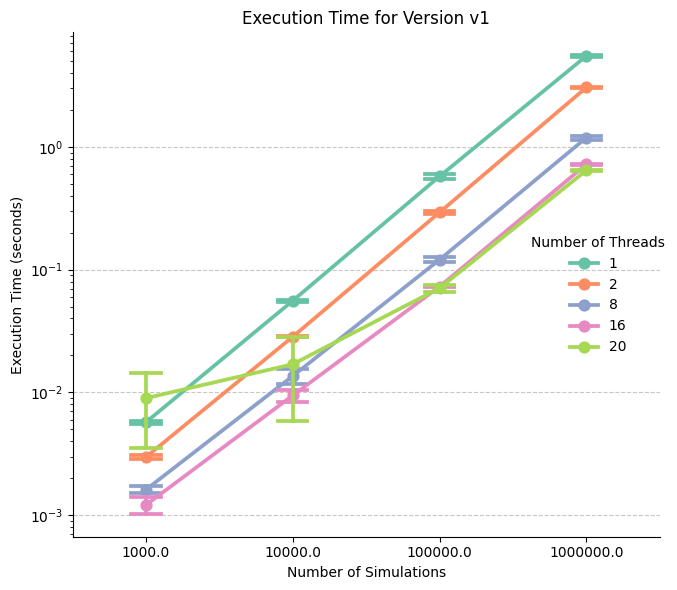
\includegraphics[width=0.8\textwidth]{cpu_exec.png}\par
\end{center}

The graph above shows the execution time depending on the number of threads available for the program.

The first thing we can see is of course that the execution time goes higher the higher the number of simulations. And, when both the x-scale and the y-scale are logarithmic, we can see that the relationship between the execution time and the number of simulations is linear, this indicates that the time is a power function of the number of simulations of the form $y=a.x^k$. However, we can see that this doesn't hold true for 20 threads.
The 20-threads executions seem to have a higher overhead that makes it slower than the 1-thread executions for a very small number of simulations like 1000.

Apart from that, the more threads we add, the faster the execution time. This also becomes true for the 20-threads variant starting from 100000 simulations, at which point it becomes better than all the other variants. This is not the case for the other variants (like 16 or 8 for example) which is rather strange.

Also, for a small number of simulations, the 20-threads variant had a higher standard deviation, meaning that the execution time varied much from one execution to another.

Our theory for the 20-threads variant is that requesting 20 threads to run in parallel at all times on a 20-cores machine is not attainable, which adds some sequential parts to the execution. For example, if we can only run 19 cores at the same time because of OS processes and run the program for 20 threads, OpenMP will have reserved some parts of the loop to execute for the 20th core. This means that, once the 19 cores have executed their part, they still need to wait for the OS to execute the 20th part of the loop.

This might not be such a problem with higher number of simulations, since it will compensate over time.

Compared with the Python implementations, the only one that was faster for 10000 simulations is the Cython implementation. Everything else was 1 or 2 orders of magnitude slower.

\section{Monte Carlo Simulation with CUDA}

To try to optimize the algorithm as much as possible, we are now going to push the code onto the graphics card using Cuda. Cuda (Compute Unified Device Architecture) is a programming model developed by NVIDIA for parallel computing on GPUs (Graphics Processing Units). 

\subsection{Main idea and challenges}

Since the Monte-Carlo simulation method is an "embarrassingly parallel" problem, we will try to leverage the extreme parallelisation allowed by the GPU. The idea is to move the intensive calculations that take place on the CPU to the GPU. As the GPU is equipped with several SMs (Scalar Multiprocessors), themselves capable of executing several hundred threads in parallel, the use of Cuda enables intensive parallelisation of calculations. We are going to use this computing power to parallelise the execution of all the simulations. 

\subsection{Implementation}

To do this, we are going to create two Cuda kernels. The first is used to initialize our random number generator. The second assigns one or more simulations to be calculated for each thread. The result of each simulation is then stored in global memory and sent back to the CPU where the final mean can be calculated. 


\begin{tcolorbox}[colback=green!5!white, colframe=green!75!black, title=Cuda random number generator]
\begin{lstlisting}[language=C++]
__global__ void setup_kernel(
    curandStatePhilox4_32_10_t *state, 
    long int random_thing
) {
    int id = threadIdx.x + blockIdx.x * blockDim.x;
    curand_init((1234 + 
        random_thing * threadIdx.x * 
        blockIdx.x * blockDim.x)%14569, 
        id, 0, &state[id]
    );
}
\end{lstlisting}
\end{tcolorbox}

\begin{tcolorbox}[colback=blue!5!white, colframe=blue!50!black, title=Cuda compute simulation]
\begin{lstlisting}[language=C++]
__global__ void generate_monte_carlo_bs(
    curandStatePhilox4_32_10_t *state,
    long int nbSim,
    int lengthSim,
    double* result,
    double K,
    double S0 = 100.0,  // Initial stock price
    double T = 1.0,     // Time to maturity (1 year)
    double r = 0.05,    // Risk-free rate (5%)
    double sigma = 0.2  // Volatility (20%)
) {
    int id = threadIdx.x + blockIdx.x * blockDim.x;
    curandStatePhilox4_32_10_t localState = state[id];

    double dt = T / lengthSim;
    double drift = (r - 0.5 * sigma * sigma) * dt;
    double diffusion = sigma * sqrt(dt);

    for (int i=id; i<nbSim; i+=blockDim.x*gridDim.x) {
        double ST = S0;
        for (int j=0; j<lengthSim; ++j) {
            double r = curand_normal_double(&localState);
            ST *= exp(drift + diffusion * r);
            state[id] = localState;
        }
        if (ST > K) {
            result[i] = ST - K;
        } else {
            result[i] = 0;
        }
    }

}
\end{lstlisting}
\end{tcolorbox}

\subsection{Results}

We benchmarked the Cuda code by running it with different numbers of simulations and measuring the time it took to finish. For each number of simulation, we ran the code 5 times and we plotted the mean execution time on the graph. Finally, we also plotted error bars, which are the standard deviation of the run times.

The GPU used for the benchmark is a laptop Nvidia A1000.

\begin{center}
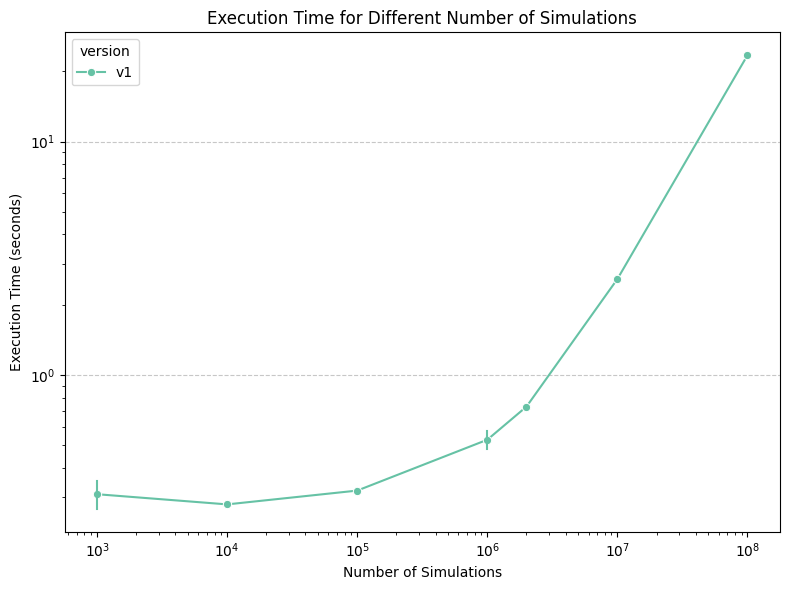
\includegraphics[width=0.8\textwidth]{gpu_benchmark.png}\par
\end{center}

As we can see on the graph, the time to execute our code with between 1000 and 100000 simulations is almost the same. This is because using the GPU comes with a fixed cost: we need to communicate with it from the CPU and moving the data also takes more time.

However, when running more than 100000 simulations the execution time begins to increase drastically. This is due to the fact that the GPU can't run all the simulations in parallel anymore and it has to do it in several chunks.

We can conclude that there is a threshold for the number of simulations below which we are under-using the GPU's parallelisation potential and above which we use its full capacity.

\subsection{Results OpenMP vs Cuda}

Now we will compare our results between our two C++ implementations: the first one using OpenMP leveraging CPU threads to parallelise our problem and the second one using Cuda to leverage the GPU's extreme parallelisation.

Do do so, we plotted our previous results on the same chart. For the CPU OpenMP results, we only kept the version with the best parameters: 16 cores.

\begin{center}
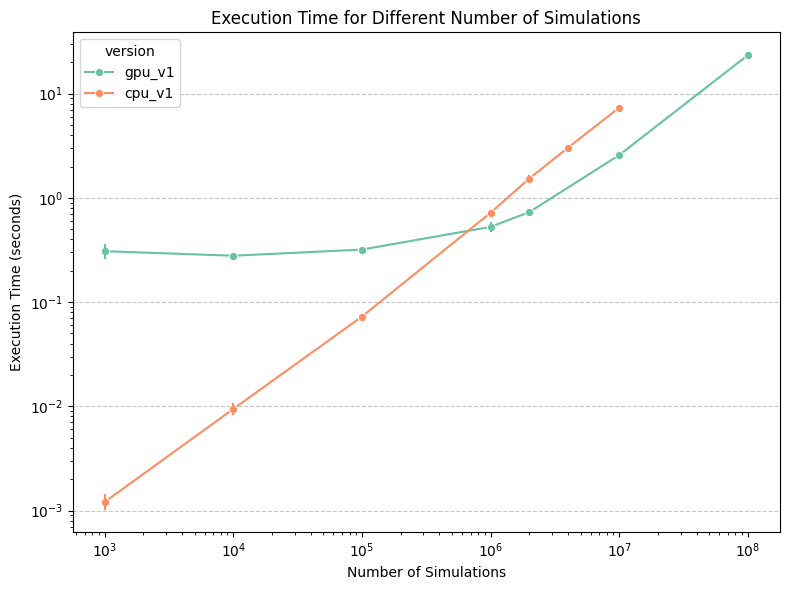
\includegraphics[width=0.8\textwidth]{gpu_vs_cpu.png}\par
\end{center}

As we anticipated, for small numbers of simulations the CPU is faster than the GPU by orders of magnitude. However, when we increase the number of simulations, the GPU becomes the fastest. This switch appears to occur at about 500000 simulations. Finally, for extremely large numbers of simulations, we can only use the GPU because the CPU is too slow.

We can conclude that for very small numbers of simulations it is not worth it to use the GPU. The GPU becomes useful for large number of simulations. 

\section{Finite Difference Methods}

\subsection{Introduction}

The objective of this project is to benchmark the performance of two implementations of the Black-Scholes finite difference methods: \texttt{optimized\_numpy} and \texttt{optimized\_numba}. These methods are tested under various configurations of grid sizes (\(M\) and \(N\)) and are evaluated for two schemes: Implicit and Crank-Nicolson. The performance metrics include mean option prices, execution times, and standard deviations of execution times.

The performance was evaluated on a 2020 MacBookPro with a Quandcore (2 Hyperthreads per core) Intel i5 processor.


\subsection{Benchmarking Results}

\subsubsection{Grid Sizes and Configurations}
\begin{itemize}
    \item \textbf{\(M\)}: Number of spatial grid points.
    \item \textbf{\(N\)}: Number of time steps.
\end{itemize}

Results are provided for various combinations of \(M\) and \(N\): \((100, 50)\), \((100, 100)\), \((100, 500)\), \((200, 50)\), \((200, 100)\), and \((200, 500)\).

\subsubsection{Results Summary}

\begin{landscape}  % Rotate the page 90 degrees
\begin{table}[h!]
    \centering
    \caption{Benchmarking Results Summary}
    \begin{tabular}{|c|c|c|c|c|c|}
        \hline
        \textbf{Grid (M, N)} & \textbf{Method} & \textbf{Scheme} & \textbf{Mean Option Price} & \textbf{Mean Execution Time (s)} & \textbf{Std Dev (s)} \\
        \hline
        \multirow{4}{*}{(100, 50)} & \multirow{2}{*}{optimized\_numpy} & Implicit & 10.1661 & 0.0072 & 0.0019 \\
         & & Crank-Nicolson & 10.1899 & 0.0081 & 0.0026 \\
         \cline{2-6}
         & \multirow{2}{*}{optimized\_numba} & Implicit & 10.1661 & 1.1745 & 3.4846 \\
         & & Crank-Nicolson & 10.1899 & 0.6724 & 1.9524 \\
        \hline
        \multirow{4}{*}{(100, 100)} & \multirow{2}{*}{optimized\_numpy} & Implicit & 10.1780 & 0.0383 & 0.0306 \\
         & & Crank-Nicolson & 10.1898 & 0.0200 & 0.0031 \\
         \cline{2-6}
         & \multirow{2}{*}{optimized\_numba} & Implicit & 10.1780 & 0.0331 & 0.0048 \\
         & & Crank-Nicolson & 10.1898 & 0.0325 & 0.0056 \\
        \hline
        \multirow{4}{*}{(100, 500)} & \multirow{2}{*}{optimized\_numpy} & Implicit & 10.1874 & 0.0852 & 0.0468 \\
         & & Crank-Nicolson & 10.1898 & 0.0742 & 0.0103 \\
         \cline{2-6}
         & \multirow{2}{*}{optimized\_numba} & Implicit & 10.1874 & 0.1301 & 0.0721 \\
         & & Crank-Nicolson & 10.1898 & 0.1240 & 0.0390 \\
        \hline
        \multirow{4}{*}{(200, 50)} & \multirow{2}{*}{optimized\_numpy} & Implicit & 10.3666 & 0.0441 & 0.0192 \\
         & & Crank-Nicolson & 10.3882 & 0.0385 & 0.0106 \\
         \cline{2-6}
         & \multirow{2}{*}{optimized\_numba} & Implicit & 10.3666 & 0.0348 & 0.0049 \\
         & & Crank-Nicolson & 10.3882 & 0.0361 & 0.0030 \\
        \hline
        \multirow{4}{*}{(200, 100)} & \multirow{2}{*}{optimized\_numpy} & Implicit & 10.3774 & 0.0579 & 0.0305 \\
         & & Crank-Nicolson & 10.3881 & 0.0469 & 0.0037 \\
         \cline{2-6}
         & \multirow{2}{*}{optimized\_numba} & Implicit & 10.3774 & 0.0490 & 0.0036 \\
         & & Crank-Nicolson & 10.3881 & 0.0582 & 0.0101 \\
        \hline
        \multirow{4}{*}{(200, 500)} & \multirow{2}{*}{optimized\_numpy} & Implicit & 10.3860 & 0.2681 & 0.0625 \\
         & & Crank-Nicolson & 10.3881 & 0.2888 & 0.0640 \\
         \cline{2-6}
         & \multirow{2}{*}{optimized\_numba} & Implicit & 10.3860 & 0.3801 & 0.0808 \\
         & & Crank-Nicolson & 10.3881 & 0.3257 & 0.0702 \\
        \hline
        \multirow{4}{*}{(400, 50)} & \multirow{2}{*}{optimized\_numpy} & Implicit & 10.4140 & 0.1346 & 0.0277 \\
         & & Crank-Nicolson & 10.4352 & 0.1771 & 0.0152 \\
         \cline{2-6}
         & \multirow{2}{*}{optimized\_numba} & Implicit & 10.4140 & 0.1046 & 0.0167 \\
         & & Crank-Nicolson & 10.4352 & 0.1583 & 0.0198 \\
        \hline
    \end{tabular}
\end{table}
\end{landscape}


\subsection{Discussion}

The benchmarking results reveal several critical insights into the performance and optimization potential of the two implementations:

\begin{itemize}
    \item \textbf{Performance Trends:} The \texttt{optimized\_numba} implementation consistently outperforms \texttt{optimized\_numpy} for larger grid sizes (\(M\) and \(N\)). The just-in-time (JIT) compilation provided by Numba optimizes execution by translating Python functions to optimized machine code at runtime, explaining the better scaling for larger configurations.
    \item \textbf{Standard Deviations:} For larger grids, \texttt{optimized\_numba} exhibits lower standard deviations in execution times, suggesting greater consistency in its performance.
    \item \textbf{Accuracy:} Both implementations yield nearly identical mean option prices, demonstrating their correctness and suitability for financial applications.
\end{itemize}

\subsection{Conclusion}

The benchmarking results demonstrate that \texttt{optimized\_numba} is more efficient for larger problems, with predictable scaling and consistent execution times. Both implementations are accurate and reliable. Further optimizations such as multithreading, GPU acceleration, and domain decomposition can enhance the scalability and performance of finite difference methods in option pricing.



% Conclusions and Future Work
\chapter{Conclusions and Future Work}
We observed through our benchmarks that parallelization for embarassingly parallel problems like the Black Scholes simulation using the Monte Carlo method quickly gives very interesting results.

Firstly, Python implementations can make use of various techniques of parallelization or even compilation (through Numba or Cython) to get more than a hundred times faster for example with Cython.

Then, the use of OpenMP for C++ implementations is straightforward and rapidly provides up to 1 order of magnitude of speedup with very little change to the code, which is useful to enable parallelization for an existing program that already works well.

Going further with CUDA, we can use massive parallelization with GPUs to get even better performance increase for higher numbers of simulations. However, the performance we obtain with the CUDA implementation is only useful starting at 5e5 simulations, due to the very high overhead of starting the GPU and loading its memory.

To conclude, parallelization of Black Scholes simulations with the Monte Carlo method gives very good results for all the different methods that we tried (both for CPU and GPU). Nevertheless, it is important to know that solutions like the CUDA implementation only become interesting when computing a very large number of simulations. In fact, it is, in this case, the only viable solution, others being too slow. Other solutions with CPU-level parallelization like OpenMP are interesting for intermediate-sized simulations, since they have a low overhead compared to the use of a GPU. OpenMP also has a simple implementation that can be interesting in situations where time and cost are of the matter.


% References
\begin{thebibliography}{9}

\bibitem{hull}
J. Hull, \textit{Options, Futures, and Other Derivatives}, 10th ed. Pearson Education, 2017.

\bibitem{panova2022}
E. Panova, V. Volokitin, A. Gorshkov, and I. Meyerov, ``Black-Scholes Option Pricing on Intel CPUs and GPUs: Implementation on SYCL and Optimization Techniques,'' in \textit{Supercomputing}, Springer International Publishing, 2022, pp. 48–62. DOI: \url{10.1007/978-3-031-22941-1_4}.

\bibitem{laszlo2015}
E. László, Z. Nagy, M. B. Giles, I. Z. Reguly, J. Appleyard, and P. Szolgay, ``Analysis of Parallel Processor Architectures for the Solution of the Black-Scholes PDE,'' in \textit{Proceedings of the 2015 IEEE International Symposium on Circuits and Systems (ISCAS)}, May 2015, pp. 1977-1980. DOI: \url{10.1109/ISCAS.2015.7169062}.

\bibitem{cvetanoska2012}
V. Cvetanoska and T. Stojanovski, ``Using High Performance Computing and Monte Carlo Simulation for Pricing American Options,'' arXiv:1205.0106 [cs.DC], 2012. Available at: \url{https://arxiv.org/abs/1205.0106}.

\end{thebibliography}



% Appendices (Optional)
\appendix
\chapter{Appendix: Mathematics and Algorithms}

\section{Monte Carlo Simulation}

Monte Carlo simulation is a stochastic approach that employs random sampling to model complex systems. For option pricing, it relies on the risk-neutral valuation principle, which states that the value of a derivative can be determined by the discounted expected payoff in a risk-neutral world.

The underlying asset price \( S \) is assumed to follow a geometric Brownian motion:
\[
dS = \mu S \, dt + \sigma S \, dz
\]
where \( \mu \) is the drift, \( \sigma \) is the volatility, and \( dz \) is a Wiener process.

In a risk-neutral world, the drift \( \mu \) is replaced by \( r \), the risk-free interest rate, and the discrete-time approximation of the process becomes:
\[
S_{t+\Delta t} = S_t \exp \left( \left( r - \frac{\sigma^2}{2} \right) \Delta t + \sigma \sqrt{\Delta t} \, Z \right)
\]
where \( Z \sim \mathcal{N}(0, 1) \) is a standard normal random variable.

The Monte Carlo simulation proceeds as follows:
\begin{enumerate}
    \item Simulate \( N \) paths for \( S \) over the life of the derivative.
    \item Calculate the payoff \( \phi(S_T) \) for each path, where \( S_T \) is the terminal stock price.
    \item Average the payoffs to estimate the expected value in a risk-neutral world:
    \[
    \mathbb{E}[ \phi(S_T) ] = \frac{1}{N} \sum_{i=1}^N \phi(S_T^{(i)})
    \]
    \item Discount this expected payoff at the risk-free rate to determine the option price:
    \[
    V = e^{-rT} \mathbb{E}[ \phi(S_T) ]
    \]
\end{enumerate}

\section{Finite Difference Method}

The finite difference method is a numerical approach to solve partial differential equations such as the Black-Scholes equation. We begin by considering the Black-Scholes PDE:
\[
\frac{\partial V}{\partial t} + \frac{1}{2} \sigma^2 S^2 \frac{\partial^2 V}{\partial S^2} + rS \frac{\partial V}{\partial S} - rV = 0,
\]
where \( V \) is the option value, \( S \) is the underlying asset price, \( \sigma \) is volatility, and \( r \) is the risk-free rate.  

We discretize the time domain into \( M \) intervals of size \( \Delta t \) and the asset price domain into \( N \) intervals of size \( \Delta S \). Using finite difference approximations, we derive three schemes:

\begin{itemize}
    \item \textbf{Explicit Scheme:} Uses a forward difference for time and central difference for space. This scheme is conditionally stable.
    \item \textbf{Implicit Scheme:} Uses a backward difference for time, requiring solving a tridiagonal system at each time step. This scheme is unconditionally stable but computationally expensive.
    \item \textbf{Crank-Nicolson Scheme:} Combines the explicit and implicit methods for second-order accuracy. It is unconditionally stable and often preferred in practice.
\end{itemize}

\subsection{Stability and Convergence Conditions}
The stability of the explicit scheme depends on the size of \( \Delta t \) and \( \Delta S \). Specifically, the Courant-Friedrichs-Lewy (CFL) condition must be satisfied to ensure convergence:
\[
\Delta t \leq \frac{\Delta S^2}{2 \sigma^2 S^2}.
\]
Implicit and Crank-Nicolson methods, being unconditionally stable, do not require such constraints.




\end{document}
